
% COMENTARIOS DE TEXTOS: NICOMÁCO DE GERASA
% Para incluír en exercicios de clase

\paragraph{\texorpdfstring{Nicómaco de Gerasa, \emph{Enchiridion
Harmonices} (ss. I-II
dC)}{Nicómaco de Gerasa, Enchiridion Harmonices (ss. I-II dC)}}\label{nicuxf3maco-de-gerasa--enchiridion-harmonices--ss.-i-ii-dc}

 \begin{quote}
  Nicómaco foi un filósofo da escola neopitagórica de fins do século I e comezos do II DC. Neste texto relátanos unha das tradicións que se conservaron sobre Pitágoras ao longo dos séculos, e que explica o descubrimento da base matemática das consonancias musicais.
 \end{quote}
 
%\begin{figure}[htp]
%\begin{center}
%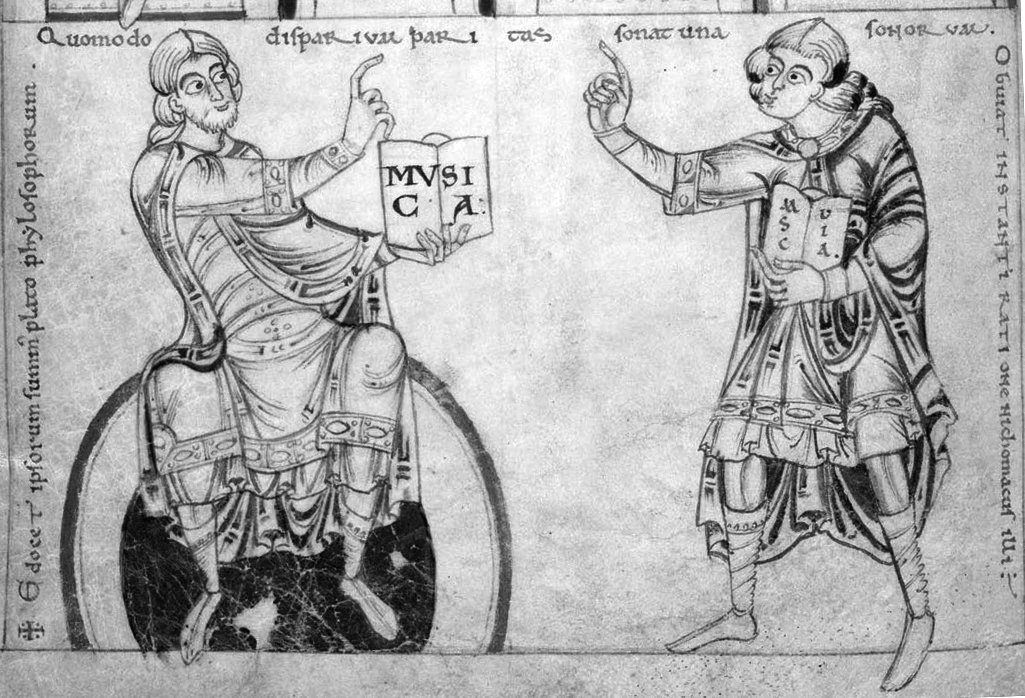
\includegraphics[width=0.45\textwidth]{/ud-01/Plato-nicomachus.jpg}
%\end{center}
%\caption{Nicomaco de Gerasa}
%\end{figure}

\begin{multicols}{3}
\setlength{\columnseprule}{1pt}
{\small
\noindent
Un día {[}\ldots{]} saíu a pasear, perdido nas súas reflexións e nos pensamentos que os seus esquemas lle suxeriron, preguntándose se podería inventar unha axuda para o oído, segura e libre de erro, como a que posúen os sentidos da vista e o tacto, un no compás, a regra, ou mesmo, podemos dicir, a dioptra; o outro nas escalas ou a invención das medidas. Sucedeu que por unha coincidencia providencial pasou xunto ao taller dun ferreiro, e ouviu alí con bastante claridade como os martelos de ferro golpeaban o yunque e emitían confusamente intervalos que, coa excepción dun, eran consonancias perfectas. Recoñeceu entre aqueles sons as consonancias de diapason (oitava), \emph{diapente} (quinta) e \emph{diatessaron} (cuarta). En canto ao intervalo entre a cuarta e a quinta, observou que era en si mesmo disonante, pero polo demais complementario da maior destas dúas consonancias. Entusiasmado, entrou no taller coma se un deus estivese a axudalo nos seus plans, e despois de varios experimentos descubriu que era a diferenza de pesos a que provocaba as diferenzas de altura, e non o esforzo dos ferreiros, nin a forma dos martelos, nin o movemento do ferro traballado. Co maior coidado, determinou os pesos dos martelos e a súa forza impulsora, que atopou perfectamente idéntica; logo volveu á súa casa.

\noindent
Fixou un só cravo no ángulo formado por dúas paredes, para evitar incluso aquí a máis lixeira diferenza, e por temor a que varios cravos, ao ter cada un a súa propia substancia, puidesen invalidar o experimento. Deste cravo colgou catro cordas idénticas en substancia,
número de fíos, espesor e torsión, e suspendeu do extremo máis baixo de cada unha delas un peso. Fixo, ademais, que a lonxitude das cordas fose exactamente a mesma, e logo, pulsándoas xuntas dúas a dúas, escoitou as consonancias arriba mencionadas que variaban con cada par de cordas. A corda estirada polo peso maior, comparada coa que soportaba o máis pequeno, daba lugar ao intervalo dunha oitava. Agora ben, a primeira representaba 12 unidades do peso dado, e a última 6. Demostrou deste xeito que a oitava está nun cociente dobre, como os pesos mesmos o fixeron sospeitar. A corda maior, comparada coa máis pequena, que representaba 8 unidades, facía soar a quinta, e probou que estaban nun cociente de sesquitercia, ao ser esa o cociente dos pesos. Logo comparouna coa seguinte, con respecto ao peso que soportaba. A máis grande das outras dúas cordas, de 9 unidades, facía soar a cuarta; así estableceu que estaba na proporción sesquitercia inversa, e que esta mesma corda estaba no cociente de sesquiáltera coa máis pequena, pois 9 a 6 é a mesma cociente, así como a segunda corda máis pequena con 8 unidades está nun cociente de sesquitercia coa de 6 unidades, e nun cociente de sesquiáltera coa de 12 unidades.

\noindent
Por conseguinte, confirmouse que o intervalo entre a quinta e a cuarta ---a cantidade pola que a quinta excede á cuarta--- está no cociente de sesquioctava, 9:8. A oitava era o sistema formado pola unión dunha e outra, a saber, a quinta e a cuarta situadas unha á beira doutra. Así, a proporción dobre componse da sesquiáltera e a sesquitercia, 12:8:6; ou, á inversa, pola unión da cuarta e a quinta, de maneira que a oitava está composta da sesquitercia e a sesquiáltera nesta orde, 12:9:6.
}

\end{multicols}


% Exercicio sobre o texto:
% ------------------------
\begin{ejercicio}[]
A quen se refire o autor de texto? \dotfill \\
Que descubre segundo o texto?\dotfill \\
Con que concepción ou teoría das vistas no punto \ref{o-pensamento-musical--na-antiguxfcidade-cluxe1sica} da páxina \pageref{o-pensamento-musical--na-antiguxfcidade-cluxe1sica} relacionas este relato? \ldots
%\par
 \vspace*{1.0cm} % espazo vertical
\end{ejercicio}
%
%
